We use MCFM NLO generator to produce the leading lepton \pt\
distributions for a number of points with non-zero anomalous
couplings. The distributions are corrected for the acceptance and
lepton reconstruction efficiency derived from a fully simulated Monte
Carlo sample. The Standard Model distribution has very few events for
large values of the leading lepton pt. It is hard to get large enough
sample of events generated with MCFM to cover this region. Therefore
we rely on the nominal Madgraph WW Monte Carlo to get the leading
lepton \pt\ distribution for the case of zero anomalous couplings. A
comparison of the distributions from different generators can be seen
in Figure~\ref{fig:generator_comparison}. It shows a good agreement
between Madgraph and MCFM distribtions.

\begin{figure}[tp]
  \centerline{
    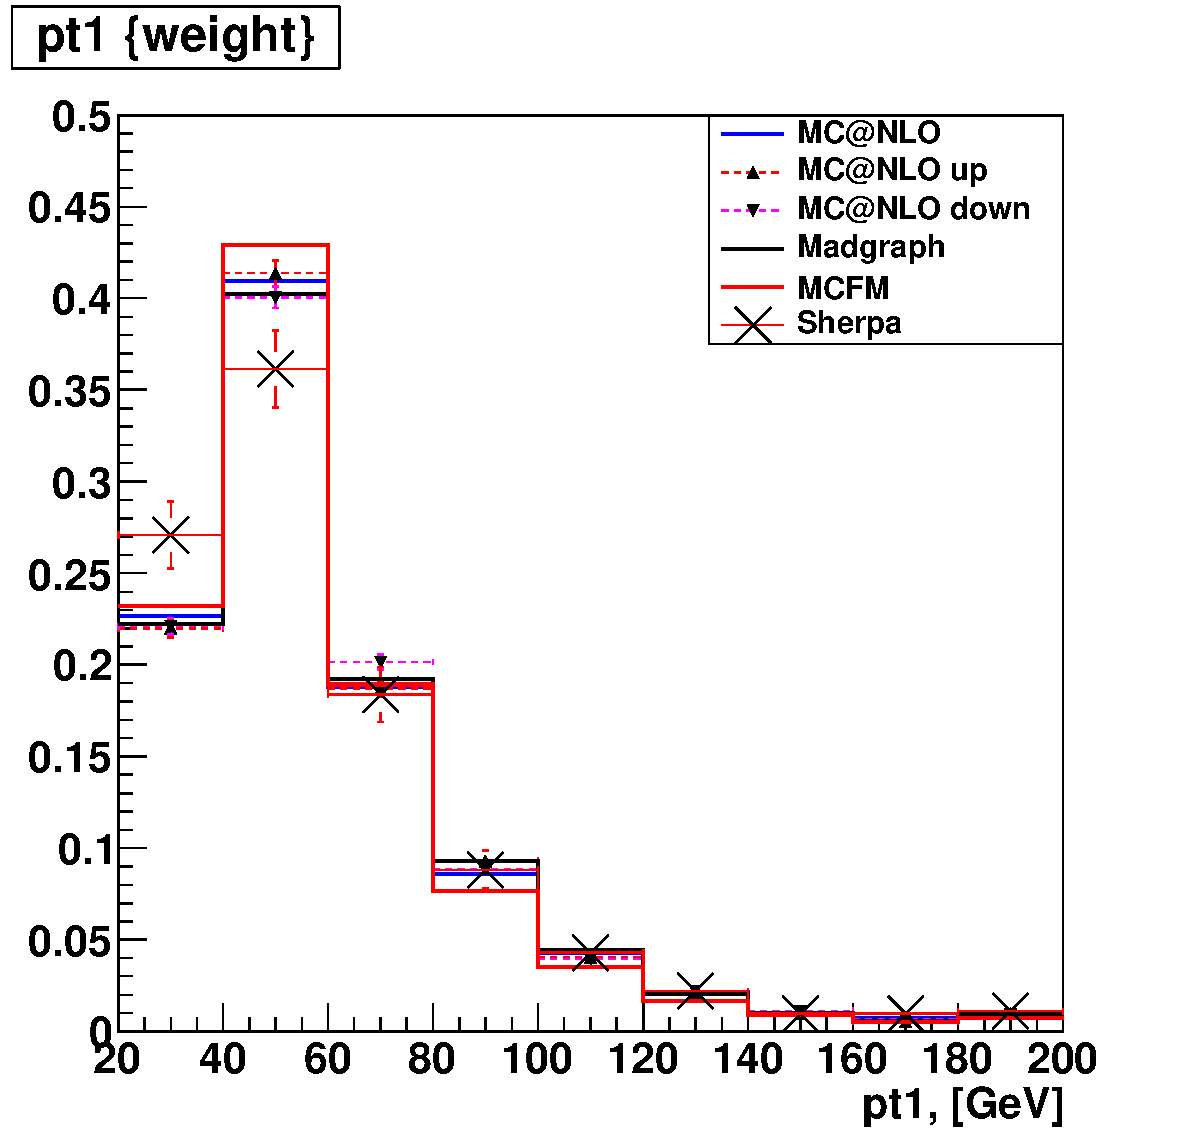
\includegraphics[width=0.6\textwidth]{figures/generator_comparison.pdf}
%    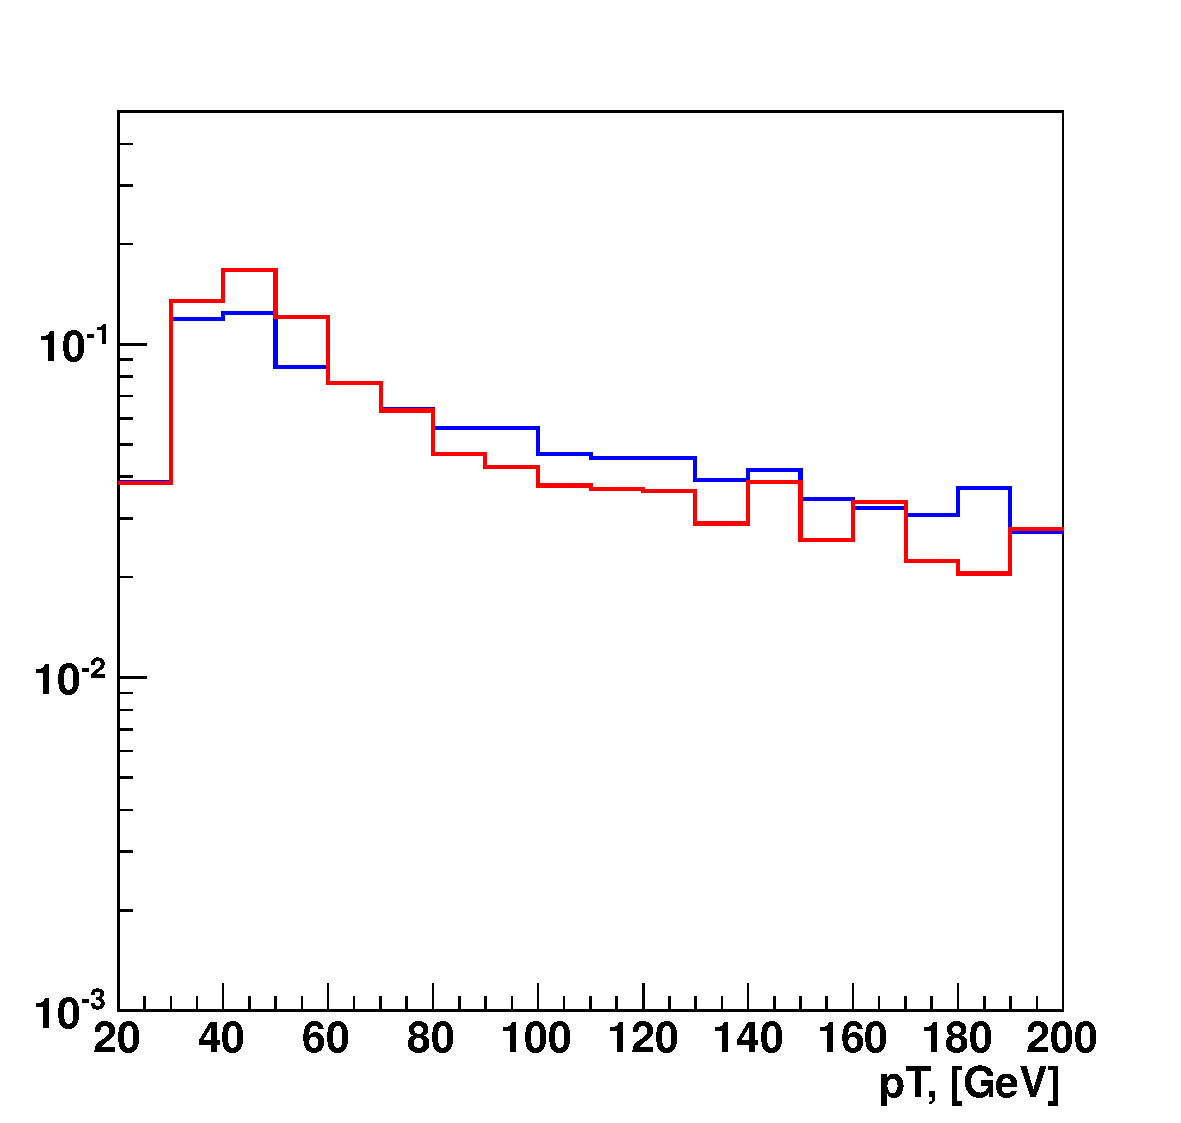
\includegraphics[width=0.45\textwidth]{figures/generator_comparison_atgc.pdf}
  }

  \caption[Generator comparison]{Leading lepton \pt\ distribution
  for \WW\ simulated data using Madgraph (full simulation), MC@NLO (full simulation),
  Sherpa (fast simulation) and MCFM (reweighted). No aTGC.}

  \label{fig:generator_comparison}
\end{figure}

It is important to confirm that all the distributions are consistent
with the model used to parametrize the leading lepton \pt\ for
arbitrary couplings. Figure~\ref{fig:pdfs} shows the result of the signal PDF
parameterization using non-parametric PDFs based on histograms. It
reveals good agreement between the initial PDFs from the
generated samples and the final aTGC model.

\begin{figure}[tp]
  \centerline{
    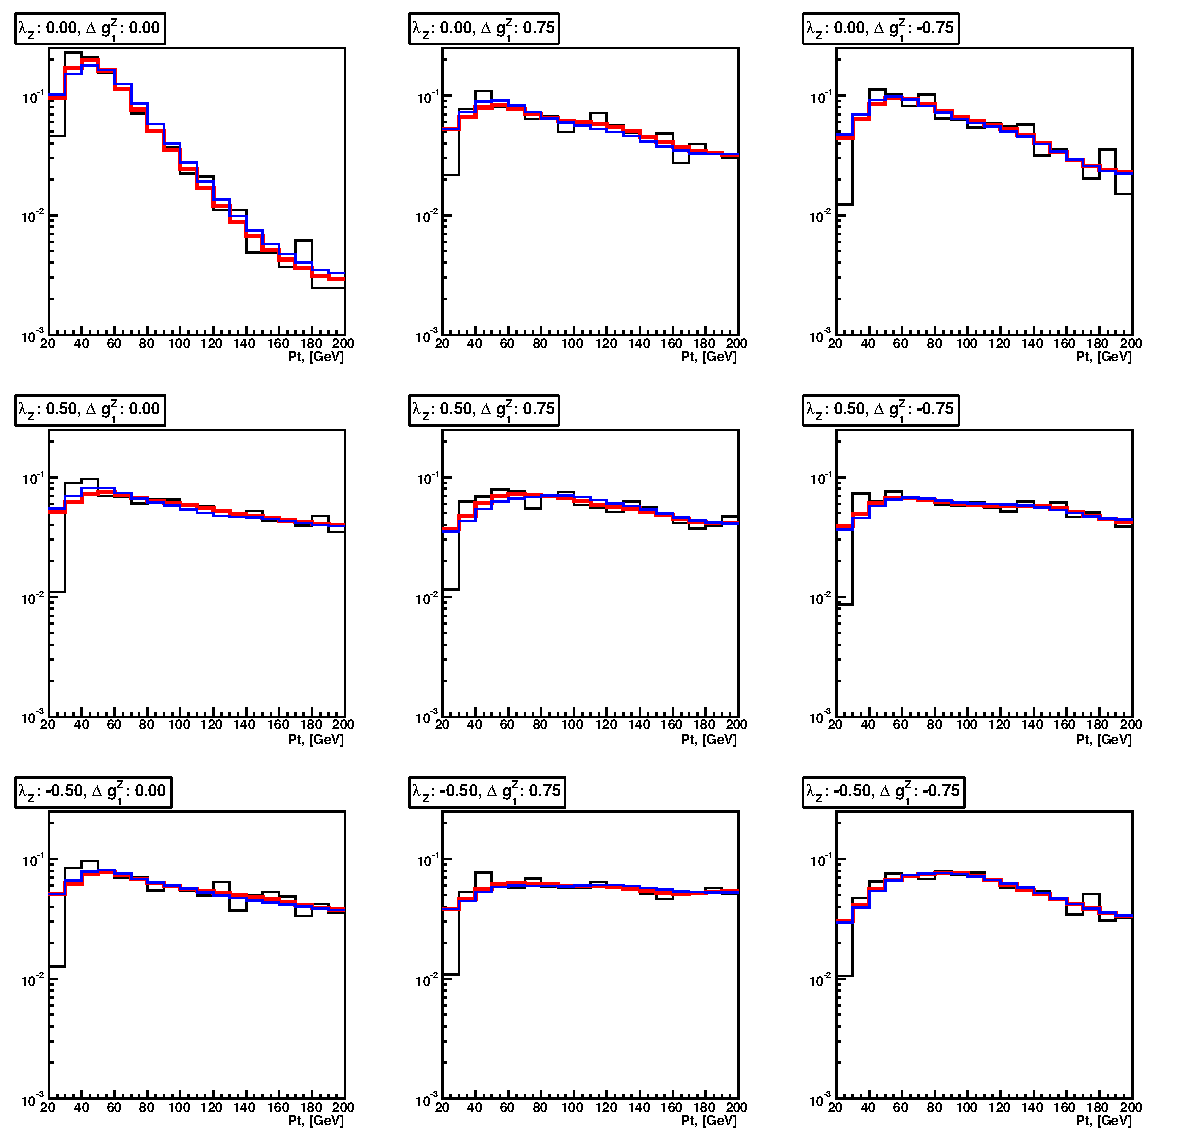
\includegraphics[width=1.0\textwidth]{figures/pdfs}
  }

  \caption[PDF parameterization] {Leading lepton \pt\ distributions
  for \ww\ events with and without aTGCs. The black points represent the
  true \pt\ distribution for Monte Carlo events that passed the final
  selection. The blue dots show the \pt\ distribution from the model used to
  parametrize the anomalous coupling effects across different values
  of the couplings.}
\label{fig:pdfs}
\end{figure}

